\renewcommand{\problemname}{B. 二维弹球}

\begin{frame}\frametitle{\problemname}
    \begin{block}{题意}
		\textbf{计算几何入门模拟题}。

		碰撞时,\textbf{沿边的方向速度不变,垂直于边方向的速度反向}。

		给定初始位置、速度向量、时间,求最终位置。
    \end{block}

	\begin{block}{出题人的话}
	计算几何好难出,凸包生成了很多 $n=20$ 的包,只能手动构造 $n=100$ 的。希望大家善待计算几何。
	\end{block}
\end{frame}

\begin{frame}\frametitle{\problemname}
\begin{block}{样例2的图示}
	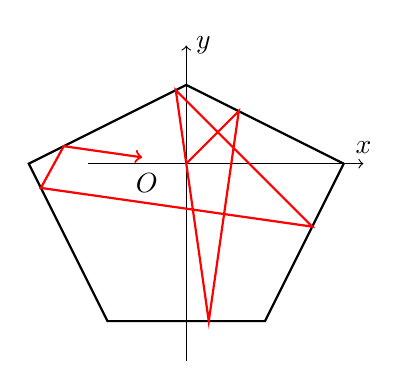
\begin{tikzpicture}[]


		\draw [->](-1.25,0) -- (2.25,0)node[above]{$x$};
		\draw [->](0,-2.5) -- (0,1.5)node[right]{$y$};
		
		\node at (-0.5,0)[below]{$O$};
		
		\draw [thick](2,0) -- (0,1) -- (-2,0) -- (-1,-2) -- (1,-2) -- (2,0); 
		
		\draw[->, red, thick] (0.000,0.000) -- (0.667,0.667) -- (0.286,-2.000) --(-0.133,0.933) -- (1.600,-0.800) -- (-1.846,-0.308) -- (-1.556,0.222) -- (-0.560,0.080);
	\end{tikzpicture}
\end{block}
\end{frame}

\begin{frame}\frametitle{\problemname}
	\begin{block}{题解}
		根据题目描述,进行模拟。

		注意到 $t\le 100$,可按时间模拟。但可能一秒钟出现多次碰撞,判断起来较为麻烦。
		
		注意到 碰撞次数 $\le 10^4$,按碰撞模拟。
		
		常用的“点+向量=点”技巧,球当前位置是一个点,速度向量与时间做数乘是下一个位置。可以用当前位置与下一个位置的连线所在的直线判断下一个碰撞点,这时需要用到的知识点是\textbf{直线交点}。
	\end{block}
\end{frame}


\begin{frame}\frametitle{\problemname}
	\begin{block}{题解}
碰撞时,\textbf{沿边的方向速度不变,垂直于边方向的速度反向}。

那么这时需要旋转速度向量。那么旋转多少度呢?求出\textbf{速度向量与边向量}的夹角 $\theta$,逆时针旋转 $2\theta$ 即可。可以证明,无论 $\theta$ 是锐角还是钝角,都是正确的。

所以我们只需要求出每一次碰撞的位置,算出碰撞间隔时间,就可以找到圆最终的位置。
	\end{block}
\end{frame}

\begin{frame}\frametitle{\problemname}
	\begin{block}{锐角的情况}

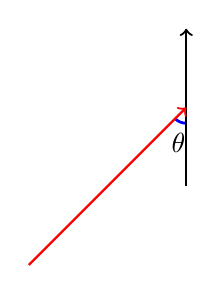
\begin{tikzpicture}[]
		
	\node at (1.9,1.8)[below]{$\theta$};
	\draw[blue,line width=1] (2,1.8) arc (270:225:.2);
	
	\draw [->,thick](2,1) -- (2,3); 
	
	\draw[->, red, thick] (0,0) -- (2,2);
\end{tikzpicture}\qquad\qquad\qquad\qquad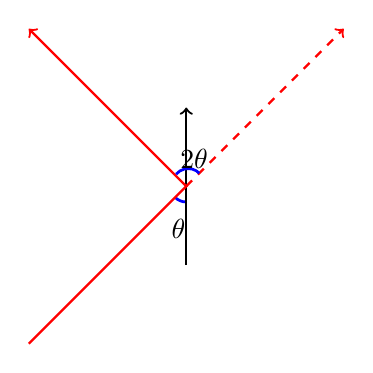
\begin{tikzpicture}[]

\node at (1.9,1.7)[below]{$\theta$};
\draw[blue,line width=1] (2,1.8) arc (270:225:.2);

\draw [->,thick](2,1) -- (2,3); 

\draw[->, red, thick] (0,0) -- (2,2) -- (0,4);

\draw[->, red, thick, dashed] (2,2) -- (4,4);
\draw[blue,line width=1] (2.166,2.166) arc (45:140:.2);
\node at (2.1,2.1)[above]{$2\theta$};
\end{tikzpicture}\end{block}
\end{frame}

\begin{frame}\frametitle{\problemname}
	\begin{block}{钝角的情况}
\begin{tikzpicture}[]
	
	\node at (1.8,2)[above]{$\theta$};
	\draw[blue,line width=1] (2.166,2.166) arc (45:180:.2);
	
	\draw [->,thick](3,2) -- (1,2); 
	
	\draw[->, red, thick] (0,0) -- (2,2);
	\draw[->, red, thick, dashed] (2,2) -- (4,4);
\end{tikzpicture}\qquad\qquad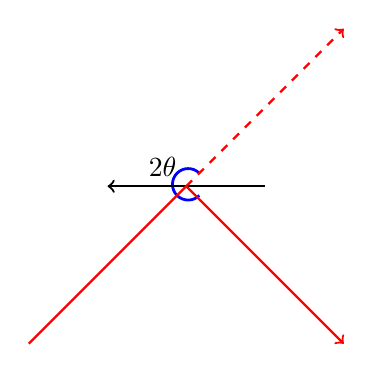
\begin{tikzpicture}[]
	
	\node at (1.7,2)[above]{$2\theta$};
	\draw[blue,line width=1] (2.166,2.166) arc (45:315:.2);
	
	\draw [->,thick](3,2) -- (1,2); 
	
	\draw[->, red, thick] (0,0) -- (2,2) -- (4,0);
	\draw[->, red, thick, dashed] (2,2) -- (4,4);
\end{tikzpicture}
\end{block}
\end{frame}
\begin{frame}\frametitle{\problemname}
	\begin{block}{题解}
		因此对一个向量 $(x,y)$,逆时针旋转 $\theta$,所得到的新向量为 $(x\cos\theta-y\sin\theta,y\cos\theta+x\sin\theta)$。

		求两线段交点比较容易,用面积法和向量去找。

		总的时间复杂度为 $O(n$碰撞次数$)$。
	\end{block}
\end{frame}
